%!TEX root = ../../master.tex
\section{Characteristics}
\noindent Resilience is related to concepts such as dependability and availability which often is measured in percentages of uptime over a time period. Bruneau and Reinhorn's \textit{"resilience triangle"} \cite[p. 21]{omer2013resilience}, describing seismic resilience in infrastructure, illustrates the same concept. A quality of service function defining how well a system is performing is plotted over time (Figure~\ref{fig:resilience_triangle}) the quality of service function being e.g. whether responses are succeeding or failing, or to what extend the latency is acceptable. A resilient system can bounce back into a fully functioning shape after a disruption.

\begin{figure}[H]
    \centering
    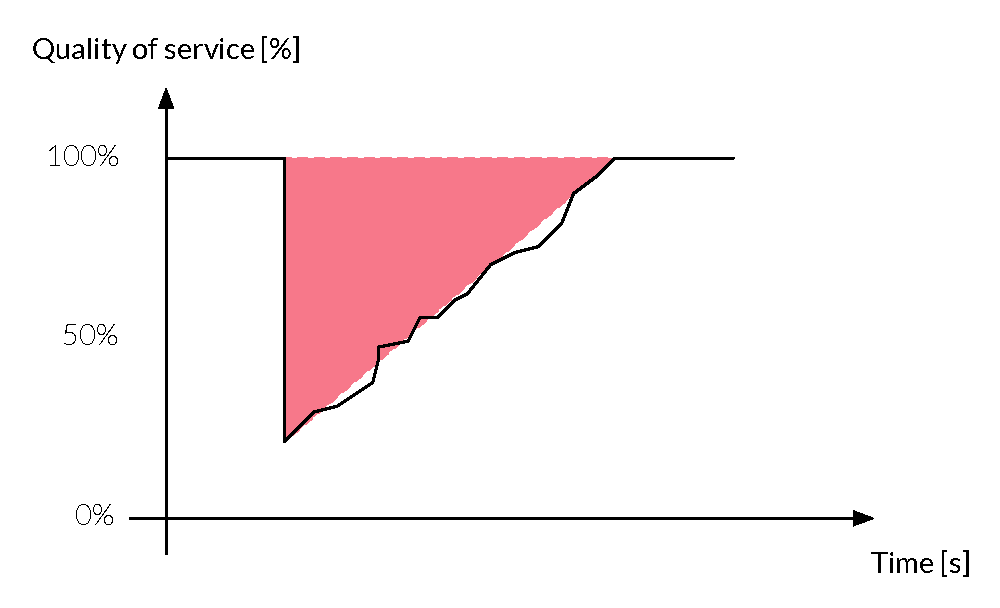
\includegraphics[width=12cm]{figures/resilience_triangle}
    \caption{Resilience Triangle}
    \label{fig:resilience_triangle}
\end{figure}

\noindent 
Quantitative metrics of resilience are difficult to find since it involves external and unpredicted disturbances. Some attempts to define metrics are: time to recovery, ratio of performance before and after a disruption, and the quality of service over time (resilience triangle) \cite[p. 21-22]{omer2013resilience}.

\noindent
Bruneau and Reinhorn define four characteristics borrowed from the domain of resilience in physical infrastructure \cite[p. 2]{bruneau_2007_seismic_resilience}.

\vspace{-4mm}
\begin{itemize}
    \setlength\itemsep{0.05em}
    \item \textbf{Robustness} is the strength to withstand stress without losing functionality 
    \item \textbf{Redundancy} is a way for the system to continue by using a substitute despite a disruption.
    \item \textbf{Resourcefulness} is the capacity to identify problems, establish priorities, and mobilize resources when a disruption happens. It can furthermore be described as the ability to recover while meeting priorities and achieving goals.
    \item \textbf{Rapidity} is the capability of containing losses, recovering functionality and avoiding future disruptions in a timely manner.
\end{itemize}

\noindent In addition to these characteristics \textit{adaptive capacity} is an important concept: \textit{"The adaptive capacity of a system can be viewed as the capacity to adapt and to reconfigure in the face of disruptions without losing functionality"} \cite[p. 25]{omer2013resilience}. Another definition involves \textit{"[...] the ability to cope with novel situations"} \cite[p. 25]{omer2013resilience}. This is in agreement with Strigini's view describing the need for techniques working in open and interconnected environments to ensure dependability.



